\documentclass{article}

% American Mathematical Society
\usepackage{amsmath}

% For \geometry{}
\usepackage{geometry}

% Set page margins
\geometry{a4paper, scale=0.8}

% Don't show the header and footer
\pagestyle{empty}

% load the tikz package
\usepackage{tikz}
\usetikzlibrary{arrows.meta}

\begin{document}
	% set the font size to large
	\large
	% set the line spacing to 3em
	\setlength{\baselineskip}{3em}
	
	% dx or d[#1]
	\renewcommand{\d}[1][x]{\ \text{d}#1}
	
	Question:
	\begin{align*}
		\int_{0}^{+\infty} e^{-x^2} \d
	\end{align*}
	
	Answer:
	
	\centering
	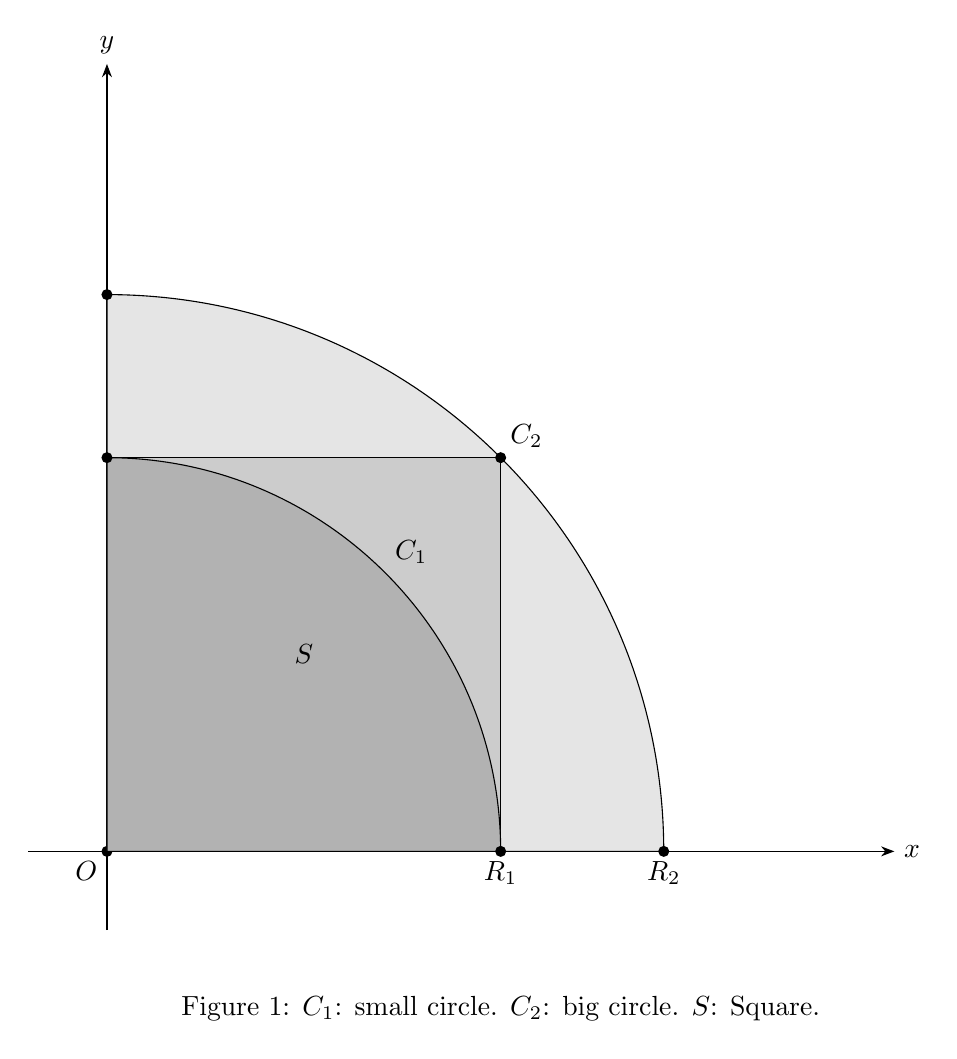
\begin{tikzpicture}[>=Stealth]
		% coordinate system
		\draw[->] (-1,0) -- (10,0) node[right] {$x$};
		\draw[->] (0,-1) -- (0,10) node[above] {$y$};
		\fill (0,0) circle (2pt) node[below left] {$O$};
		
		% shapes
		\filldraw[fill=black!10!white, draw=black] (0,0) -- (7.071067,0) arc[start angle=0, end angle=90, radius=7.071067] -- cycle;
		\filldraw[fill=black!20!white, draw=black] (0,0) rectangle +(5,5);
		\filldraw[fill=black!30!white, draw=black] (0,0) -- (5,0) arc[start angle=0, end angle=90, radius=5] -- cycle;
		\fill (5,0) circle (2pt) node[below] {$R_1$};
		\fill (7.071067,0) circle (2pt) node[below] {$R_2$};
		\fill (0,5) circle (2pt);
		\fill (0,7.071067) circle (2pt);
		\fill (5,5) circle (2pt);
		\node at (5/2,5/2) {$S$};
		\node[above right] at (45:5) {$C_1$};
		\node[above right] at (45:7.071067) {$C_2$};
		
		% text
		\node at (5,-2) {Figure 1: $C_1$: small circle. $C_2$: big circle. $S$: Square.};
	\end{tikzpicture}
	
	\begin{align*}
		& let
		\\
		& \quad f(x, y) = e^{- x^2 - y^2}
		\\
		& because
		\\
		& \quad R_2 = \sqrt{2} R_1
		\\
		& therefore
		\\
		& \quad \iint_{C_1} f(x, y) \d[x] \d[y] & & \le \iint_{S} f(x, y) \d[x] \d[y] && \le \iint_{C_2} f(x, y) \d[x] \d[y]
		\\
		& \quad \iint_{C_1} e^{- x^2 - y^2} \d[x] \d[y] & & \le \int_{0}^{R_1} e^{-x^2} \d[x] \cdot \int_{0}^{R_1} e^{-y^2} \d[y] && \le \iint_{C_2} e^{- x^2 - y^2} \d[x] \d[y]
		\\
		& \quad \frac{\pi}{4} (1 - e^{-R_1^2}) & & \le \left( \int_{0}^{R_1} e^{-x^2} \d[x] \right)^2 && \le \frac{\pi}{4} (1 - e^{-2 R_1^2})
		\\
		& \quad \lim_{R_1 \to +\infty} \frac{\pi}{4} (1 - e^{-R_1^2}) & & \le \lim_{R_1 \to +\infty} \left( \int_{0}^{R_1} e^{-x^2} \d[x] \right)^2 && \le \lim_{R_1 \to +\infty} \frac{\pi}{4} (1 - e^{-2 R_1^2})
		\\
		& \quad \frac{\pi}{4} & & \le \left( \int_{0}^{+\infty} e^{-x^2} \d[x] \right)^2 && \le \frac{\pi}{4}
		\\
		& therefore
		\\
		& \quad \int_{0}^{+\infty} e^{-x^2} \d[x] = \frac{\sqrt{\pi}}{2}
	\end{align*}
\end{document}
